\spacing{1.3}


\section{Introducción}


\begin{definition}[Termodin\'amica]
    Se denomina \textbf{termodinámica} a la parte de la física que estudia los intercambios de calor y trabajo que acompañan a los procesos fisicoquímicos; si estos son reacciones químicas, la parte de la ciencia que los estudia se denomina \textbf{termoquímica}
\end{definition}


\section{Termodinámica. Conceptos básicos}\label{sec:termodinamica.-conceptos-basicos}

\subsection{Equivalente mecánico del calor}\label{subsec:equivalente-mecanico-del-calor}

\textbf{James Prescott Joule} diseñó un dispositivo que permitía efectuar medidas muy precisas de la equivalencia entre el trabajo mecánico y el calor.

\begin{itemize}
    \item La caída de las pesas (trabajo mecánico) produce la fricción interna de las paletas con el agua (entra calor al sistema), lo que provoca un aumento de temperatura de esta.
    \item Joule demostró que, cuando entra \SI{1}{\calorie} de calor, las pesas hacen \num{4.184} unidades de trabajo mecánico que más tarde, y en su honor, se denominaron julios (\unit{\joule}).
\end{itemize}

Podemos decir, por tanto, que \(\SI{1}{\calorie} = \SI{4.18}{\joule}\)

\subsection{Sistema termodinámico}\label{subsec:sistema-termodinamico}

Se llama \textbf{sistema termodinámico} aquella parte del \textbf{universo} que aislamos para someterla a un estudio fisicoquímico.
Lo que rodea a este sistema recibe el nombre de \textbf{entorno}.

Según sea la relación entre sistema y entorno tendremos:

\begin{enumerate}[label=\numberballmDarkTeal]
        \item \textbf{Sistema abierto}.
        Intercambia materia y energía con el entorno.
        \item \textbf{Sistema cerrado}.
        Intercambia energía con el entorno, pero no materia.
        \item \textbf{Sistema aislado}.
        No intercambia materia ni energía con el entorno.
\end{enumerate}

\begin{figure}[H]
    \centering
    % [FIGURA ORIGINAL] \includegraphics[scale=.7]{images/imagesUD4Termidonamica/UD4_Teoria/sistemas}\label{fig:sistemas}
    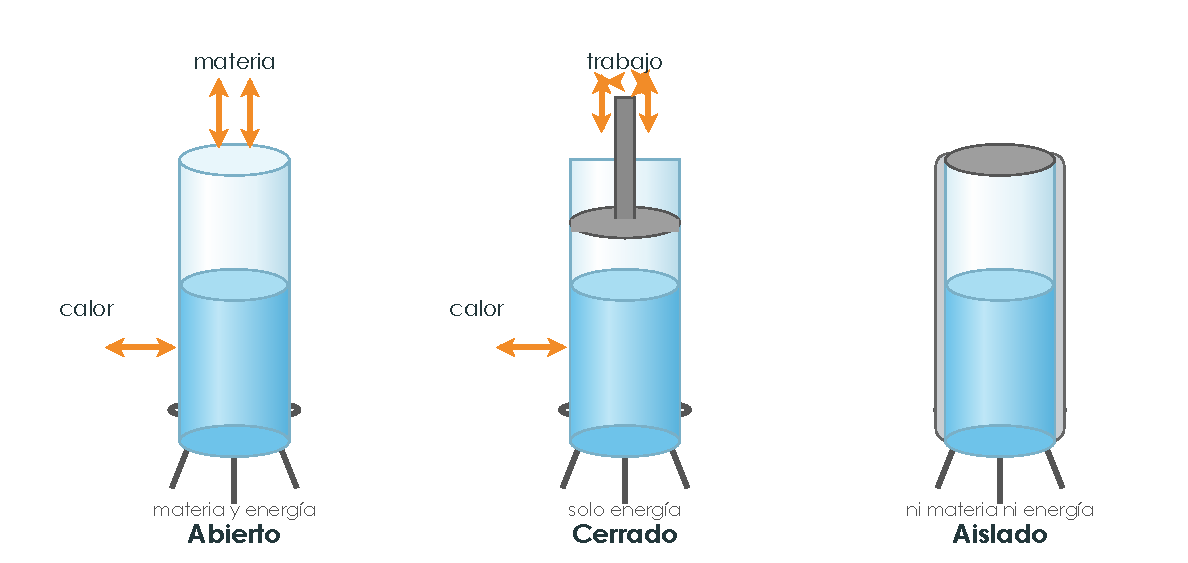
\includegraphics[width=0.75\linewidth]{FigurasSVG/UD4_Termodinamica/pdf/UD4_01_sistemas.pdf}\label{fig:sistemas}
\end{figure}

Para describir un sistema termodinámico es preciso conocer el valor de sus propiedades.
A estas propiedades / magnitudes se les conoce como \textbf{variables termodinámicas} como por ejemplo el volumen, temperatura, presión, composición etc.

Algunas variables dependen solo del estado en que se encuentra el sistema y no de cómo evolucionó para llegar a él, como el volumen, la presión o la temperatura.
A este tipo de variables se les denomina \textbf{variables de estado} o \textbf{funciones de estado}.

A las variables que dependen de como evoluciona el sistema se les conoce como \textbf{variables de transferencia} como puede ser el calor, trabajo, etc.

\subsection{Procesos termodinámicos}\label{subsec:procesos-termodinamicos}


\begin{definition}[Poceso termodinámico]
    Se denomina \textbf{proceso termodinámico} a la evolución seguida por un sistema cuando pasa de un estado inicial (\(p_0, T_0, V_0\)) a otro final (\(p_f, T_f, V_f\)).
\end{definition}


Estos procesos termodinámicos se clasifican en:

\begin{enumerate}[label=\numberballmDarkTeal]
        \item Atendiendo al sentido de la evolución:
        \begin{itemize}
            \item \textbf{Irreversibles}: si lo hacen en un único sentido.
            La mayor parte de los procesos son de este tipo:
            \begin{equation*}
                \ch{4 Fe + 3 O2 -> 2 Fe2O3}
            \end{equation*}
            \item \textbf{Reversibles}: si lo hacen a través de múltiples estados de equilibrio.
            \begin{equation*}
                \ch{N2 + 3 H2 <=> 2 NH3}
            \end{equation*}
        \end{itemize}
        \item Atendiendo a si en la evolución hay alguna variable de estado que permanezca constante:
        \begin{itemize}
            \item \textbf{Isobáricos}: si la presión no varía.
            La mayoría de las reacciones químicas se hacen a presión constante puesto que se realizan en recipientes abiertos.
            \item \textbf{Isocóricos}: si el volumen no varía.
            Ocurre en recipientes cerrados.
            \item \textbf{Isotérmicos}: si la temperatura no varía.
        \end{itemize}
\end{enumerate}


\section{Calor y trabajo en un proceso}\label{sec:calor-y-trabajo-en-un-proceso}

\subsection{Intercambio de calor en un proceso}\label{subsec:intercambio-de-calor-en-un-proceso}


\begin{definition}[Calor]
    Se define \textbf{calor} (\(\bm{Q}\)) como aquella energía en tránsito (intercambiada entre el sistema y su entorno) que produce cambios de temperatura o cambios de estado.
\end{definition}


El cálculo del calor variará si existen cambios de temperatura o cambios de estado:

\begin{itemize}
    \item Si existe cambio de temperatura:

    \begin{centeredequation}
        Q = m\ c_e\ \Delta T
    \end{centeredequation}

    Donde \(c_e\) es el llamado \textbf{calor específico} que nos dice la relación entre el calor agregado por unidad de masa y la variación de la temperatura que en ella se produce y es característico de cada sustancia.
    Sus unidades son \unit{\joule\per\kilo\g} o \unit{\calorie\per\g\per\celsius} y \(\Delta T\) es el incremento de temperatura experimentado.
    \item Si existe un cambio de estado:

    \begin{centeredequation}
        Q = m\ L_{\text{fus}} \qquad  Q = m\ L_{\text{vap}}
    \end{centeredequation}

    donde \(L_{\text{fus}}\) o \(L_{\text{vap}}\) son los llamados \textbf{calor latente de cambio de estado} siendo el primero para el cambio de sólido a líquido y el segundo de líquido a gas.
    Este calor latente de cambio de estado se define como la cantidad de calor que hay que suministrar a la unidad de masa de una sustancia para que, sin variar su temperatura, cambie de estado, midiéndose, por tanto, en \unit{\joule\per\kilo\g} o \unit{\calorie\per\g}
\end{itemize}

\subsection{Intercambio de trabajo en un proceso}\label{subsec:intercambio-de-trabajo-en-un-proceso}

Se define \textbf{trabajo} (\(\bm{W}\)) como aquella energía en tránsito que sucede a través de fuerzas y desplazamientos.
Su unidad sería \unit{\joule} o \unit{\atmosphere\litre}.

La relación del julio con el \unit{\atmosphere\litre}:
\begin{centeredequation}
    \SI{1}{\atmosphere\litre} = \SI{101300}{\pascal}\cdot \SI{e-3}{\cubic\metre} = \SI{101.3}{\joule}
\end{centeredequation}

Según el criterio de signos:

\begin{itemize}
    \item Si \(W<0\) el trabajo lo \textbf{realiza el sistema}.
    \item Si \(W>0\) el trabajo lo \textbf{realiza el entorno}.
\end{itemize}

En las reacciones químicas el trabajo está relacionado con las expansiones y compresiones.

\begin{itemize}
    \item El trabajo en una expansión:
    \begin{gather*}
        dW = -F\ dx = -p\ S\ dx = -p\ dV \separ
        W = - \int_{V_1}^{V_2} p\ dV
    \end{gather*}
    \item El trabajo en una compresión:
    \begin{gather*}
        dW = F\ dx = p\ S\ dx = p\ dV \separ
        W =  \int_{V_1}^{V_2} p\ dV
    \end{gather*}
\end{itemize}

Para resolver las integrales, es preciso conocer como varía la \(p\) en función del \(V\).
Según el tipo de proceso tendremos que:

\begin{itemize}
    \item \textbf{Isobáricos} (\(p = \text{cte}\))
    \begin{gather*}
        W = - \int_{V_1}^{V_2} p\ dV = - p \int_{V_1}^{V_2}  dV \separ
        W = -p\ (V_2 - V_1)
    \end{gather*}
    \begin{figure}[H]
        \centering
        % [FIGURA ORIGINAL] \includegraphics[scale=1]{images/imagesUD4Termidonamica/UD4_Teoria/trabajo_isobarico}\label{fig:trabajo-isobarico}
        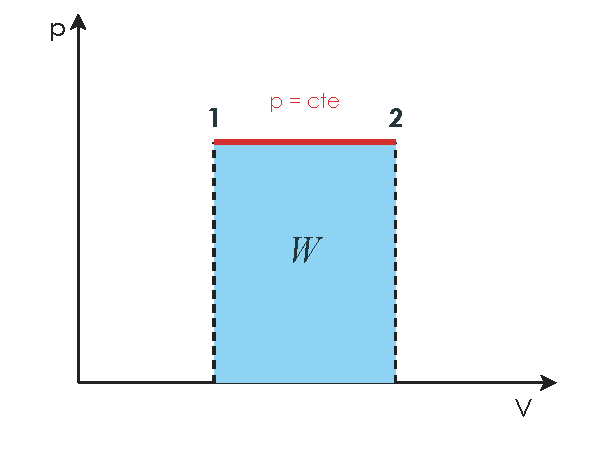
\includegraphics[width=0.45\linewidth]{FigurasSVG/UD4_Termodinamica/pdf/UD4_02_trabajo_isobarico.pdf}\label{fig:trabajo-isobarico}
    \end{figure}
    \item \textbf{Isotérmicos} (\(T = \text{cte}\))
    \begin{gather*}
        W = - \int_{V_1}^{V_2} p\ dV = - \int_{V_1}^{V_2} \dfrac{n\ R\ T}{V} \ dV = - n\ R\ T \int_{V_1}^{V_2} \dfrac{dV}{V} \separ
        W = -n\ R\ T\ ln\ \dfrac{V_2}{V_1}
    \end{gather*}
    \begin{figure}[H]
        \centering
        % [FIGURA ORIGINAL] \includegraphics[scale=1]{images/imagesUD4Termidonamica/UD4_Teoria/trabajo_isotermico}\label{fig:trabajo-isotermico}
        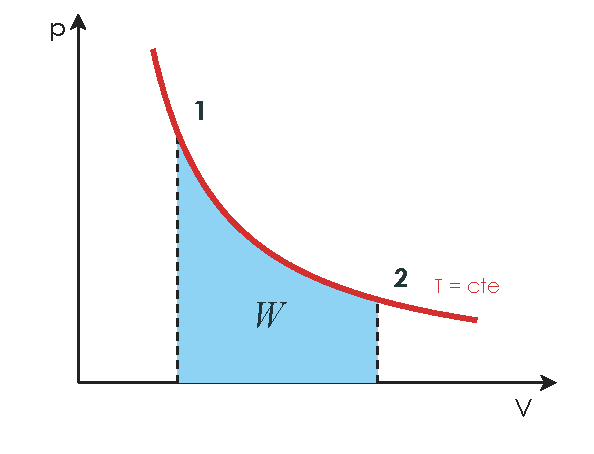
\includegraphics[width=0.45\linewidth]{FigurasSVG/UD4_Termodinamica/pdf/UD4_03_trabajo_isotermico.pdf}\label{fig:trabajo-isotermico}
    \end{figure}
    \item \textbf{Isocóricos} (\(V = \text{cte}\)).
    En este caso al no existir variación de volumen el \(V_2 = V_1\) y por tanto el trabajo será \(W = 0\)
    \begin{equation*}
        W = - \int_{V_1}^{V_2} p\ dV = 0
    \end{equation*}
    \begin{figure}[H]
        \centering
        % [FIGURA ORIGINAL] \includegraphics[scale=1]{images/imagesUD4Termidonamica/UD4_Teoria/trabajo_isocorico}\label{fig:trabajo-isocorico}
        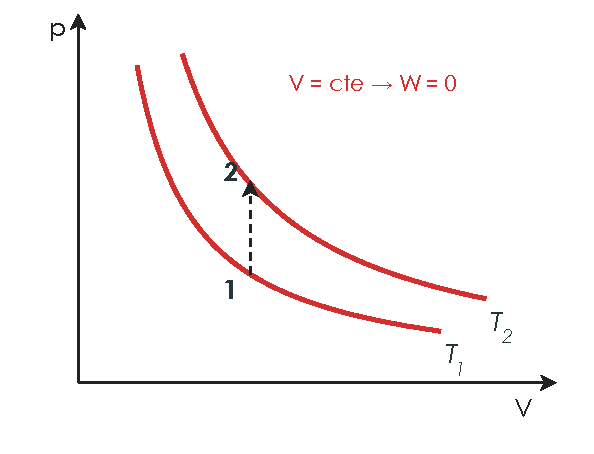
\includegraphics[width=0.45\linewidth]{FigurasSVG/UD4_Termodinamica/pdf/UD4_04_trabajo_isocorico.pdf}\label{fig:trabajo-isocorico}
    \end{figure}
\end{itemize}


\section{Primer principio de la termodinámica}\label{sec:primer-principio-de-la-termodinamica}

Cuando un sistema experimenta una transformación, suele intercambiar calor y trabajo con su entorno; el resultado es una variación de su \textbf{energía interna}

\begin{center}
    \begin{definition}[Energía Interna]
        La \textbf{energía interna} de un sistema es la suma de las energías de todas las partículas que lo forman.
        Se representa con la letra \(U\) y en el sistema internacional se mide en \textbf{julios}.
        Es una función de estado ya que su valor solo depende del estado en el que se encuentra el sistema.
    \end{definition}
\end{center}



\begin{figure}[H]
    \centering
    % [FIGURA ORIGINAL] \includegraphics[scale=1]{images/imagesUD4Termidonamica/UD4_Teoria/energia_interna}
    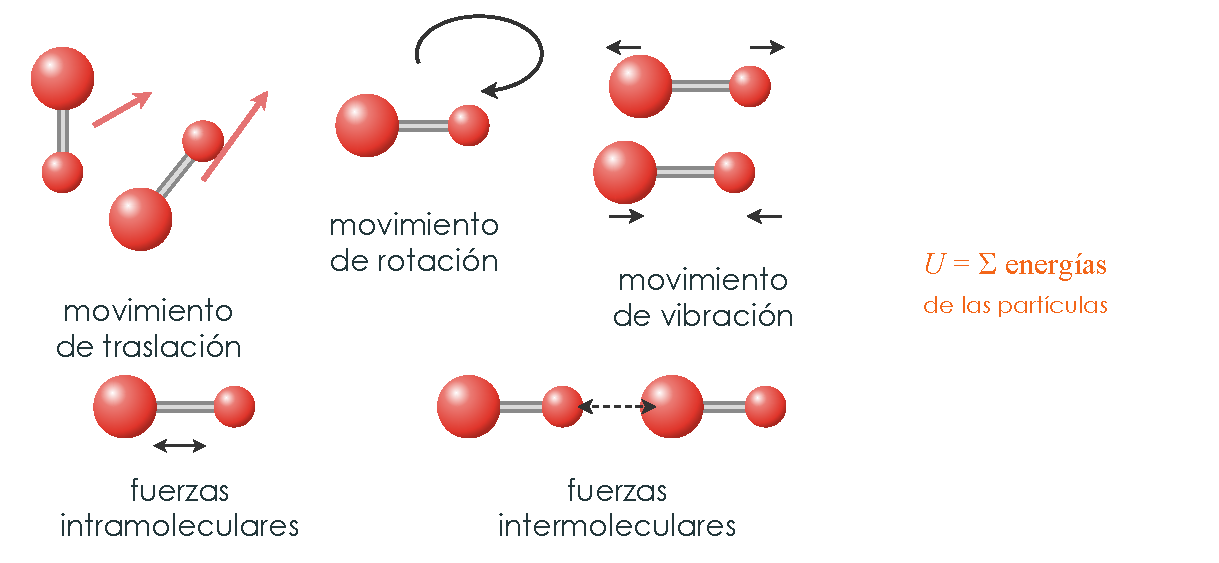
\includegraphics[width=0.8\linewidth]{FigurasSVG/UD4_Termodinamica/pdf/UD4_05_energia_interna.pdf}
    \caption{Representación de la energía interna}
    \label{fig:energia_interna}
\end{figure}

Las partículas de un sistema tienen energía cinética (por el movimiento de las moléculas) y energía potencial (por la atracción entre electrones y núcleos dentro de una molécula y las interacciones entre las moléculas).

\begin{ley}[Primer Principio de la Termodinámica]
    El \textbf{Primer principio de la Termodinámica} establece que, cuando un sistema evoluciona de un estado inicial a otro final, la variación que experimenta su energía interna coincide con la suma del calor y trabajo que intercambia con el entorno en esa transformación:
    \begin{centeredequation}
        \Delta U = Q + W
    \end{centeredequation}

\end{ley}


Si nos fijamos, este primer principio no es más que una conservación de la energía.

Es importante conocer los \textbf{criterios de signos} que recomienda la IUPAC para el calor y el trabajo que intercambia un sistema con su entorno.

\begin{itemize}
    \item Si se transfiere calor o trabajo desde el entorno al sistema consideraremos \(Q>0\) y \(W>0\).
    \item Si es el propio sistema el que cede calor o trabajo al entorno, entonces consideraremos \(Q<0\) y \(W<0\).
\end{itemize}

\begin{figure}[H]
    \centering
    % [FIGURA ORIGINAL] \includegraphics[scale=1]{images/imagesUD4Termidonamica/UD4_Teoria/criteriosdesignos}
    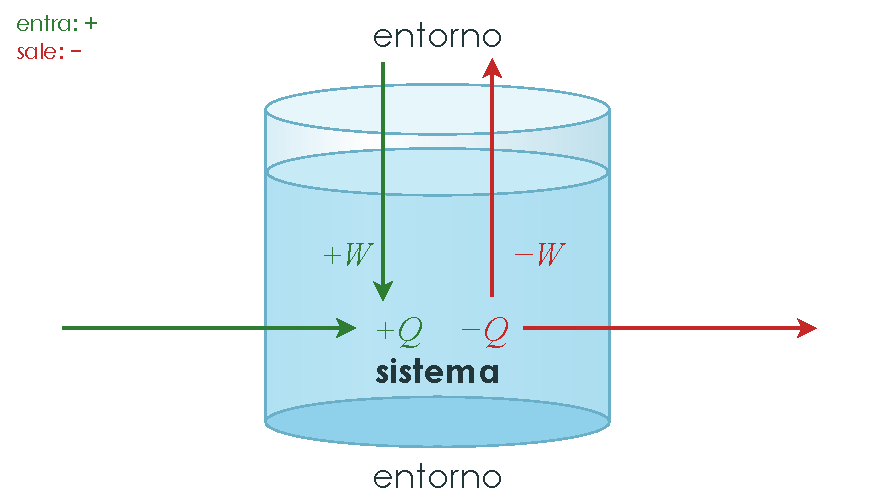
\includegraphics[width=0.6\linewidth]{FigurasSVG/UD4_Termodinamica/pdf/UD4_06_criterio_signos.pdf}
    \caption{Criterio de signos}
    \label{fig:cristerio-de-signos}
\end{figure}

\subsection{Aplicación del primer principio a diversos procesos termodinámicos}\label{subsec:aplicacion-del-primer-principio-a-diversos-procesos-termodinamicos.}

\begin{enumerate}[label=\numberballmDarkTeal]
        \item \textbf{Proceso isotérmico} (\(T = \text{cte}\)).
        En este caso, \(\Delta U = 0\) ya que la energía interna solo depende de la temperatura y, al ser esta constante, su variación es \num{0}.
        Si aplicamos el primer principio llegamos a la conclusión de que \(Q = - W\).
        \begin{gather*}
            \Delta U = Q + W \Rightarrow 0 = Q + W \separ
            Q = -W
        \end{gather*}
        \item \textbf{Proceso adiabático}.
        Es aquel en el que no hay intercambio de calor con el entorno (\(Q = 0\)). Aplicando el primer principio tendríamos:
        \begin{gather*}
            \Delta U = Q + W \Rightarrow \Delta U = 0 + W \separ
            \Delta U = W
        \end{gather*}
        Por lo tanto de aquí podemos determinar que si un gas se expande disminuirá su energía interna (\(\Delta U < 0\)) puesto que \(W < 0\).
        Si un gas se comprime aumentará su energía interna (\(\Delta U > 0\)) puesto que \(W > 0\).
        \item \textbf{Proceso isocórico} (\(V = \text{cte}\)).
        En este caso el trabajo será \(W = 0\) puesto que no hay cambio en el volumen (\(W = -p\ dV\)). Si aplicamos el primer principio tendremos que:
        \begin{gather*}
            \Delta U = Q + W \Rightarrow \Delta U = Q + 0 \separ
            \Delta U = Q
        \end{gather*}
        En este caso vemos como la variación de energía interna es igual al calor puesto en juego en el proceso.
        Por norma general en este caso se suele representar el calor como \(Q_V\) para indicar que es a volumen constante.
        \begin{centeredequation}
            \Delta U = Q_V
        \end{centeredequation}

        \item \textbf{Proceso isobárico} (\(p = \text{cte}\)).
        Aplicando el primer principio tendremos que:
        \begin{centeredequation}
            \Delta U = Q + W \Rightarrow \Delta U = Q_p - p\ \Delta V
        \end{centeredequation}

        Como vemos en este caso, el calor lo hemos denominado \(Q_p\) para indicar que estamos en un proceso a \(p = \text{cte}\).
\end{enumerate}


\section{Entalpía. Ecuaciones termoquímicas}\label{sec:entalpia.-ecuaciones-termoquimicas}

Por norma general, las reacciones químicas transcurren a presión constante.
Si aplicamos el primer principio a esta situación tendríamos que:
\begin{centeredequation}
    \Delta U = Q_p - p\ (V_2-V_1) \Rightarrow U_2-U_1 = Q_p - p\ (V_2-V_1)
\end{centeredequation}
Si reordenamos la expresión de manera que:
\begin{centeredequation}
(U_2 + pV_2) -  (U_1 + pV_1) = Q_p \label{eq:definicion_entalpia}
\end{centeredequation}

Podemos definir una función que denominamos \textbf{entalpía} y la representamos con la letra \(\bm{H}\) de la siguiente manera:
\begin{centeredequation}
    H = U + pV
\end{centeredequation}

De esta manera, la expresión de la ecuación~\eqref{eq:definicion_entalpia} quedará como:
\begin{centeredequation}
    Q_p = H_2 - H_1 = \Delta H
\end{centeredequation}


\begin{center}
    \begin{definition}[Entalp\'ia]
        Se denomina  \textbf{entalpía} de un sistema (\(H\)) a la magnitud suma de la energía interna y el producto de la presión por el volumen de dicho sistema \(H = U + pV\).
        Es una función de estado y su unidad es el julio.

        La entalpía, por tanto, representa el calor que intercambia con el entorno cuando el proceso se realiza a presión constante.
    \end{definition}
\end{center}

\subsection{Relación ente \texorpdfstring{\(\Delta U\)}{U} y \texorpdfstring{\(\Delta H\)}{H}}\label{subsec:relacion-ente-texorpdfstring{(delta-u)}{u}-y-texorpdfstring{(delta-h)}{h}}

Es posible establecer la relación entre la variación de entalpía y la de energía interna utilizando la propia definición de entalpía vista anteriormente.
\begin{centeredequation}
    H = U + pV \Rightarrow \Delta H = \Delta U + \Delta (pV)
\end{centeredequation}

\begin{itemize}
    \item Si en el sistema solo intervienen \textbf{sólidos} o \textbf{líquidos}, la presión y el volumen prácticamente no varían siendo, por tanto, el trabajo de expansión cero.
    En esos casos:
    \begin{gather}
        \Delta H = \Delta U \notag \separ
        Q_p = Q_v
    \end{gather}
    \item Si en el sistema intervienen \textbf{gases ideales}:
    \begin{gather}
        \Delta H = \Delta U + \Delta (nRT) = \Delta U + (\Delta n)RT \notag \separ
        Q_p = Q_v + (\Delta n) R T
    \end{gather}
\end{itemize}

\subsection{Ecuación termoquímica}\label{subsec:ecuacion-termoquimica}

La ecuación termoquímica es la ecuación química ajustada en la que, además de indicar el estado de agregación de todas las sustancias que intervienen y la presión y la temperatura a la que se realiza, hay que especificar la cantidad de calor intercambiado con el entorno.
\begin{centeredequation}
    \ch{1/2 N2 \gas{} + 1/2 O2 \gas{} -> NO \gas{}}\quad  \Delta H^0 = \energia[kj]{90.2}
\end{centeredequation}

Según el signo de este calor puesto en juego tendremos reacciones \textbf{endotérmicas} o \textbf{exotérmicas}

\begin{itemize}
    \item Si para pasar de reactivos a productos el sistema cede calor al entorno, el proceso se denomina \textbf{exotérmico} y \(\Delta H < 0\).
    \item Si para pasar de reactivos a productos el sistema absorbe calor del entorno, el proceso se llama \textbf{endotérmico} y \(\Delta H > 0\).
\end{itemize}

\subsection{Diagramas entálpicos}\label{subsec:diagramas-entalpicos}

Los diagramas entálpicos son la representación gráfica del contenido energético de los reactivos (\textbf{R}), los productos (\textbf{P})  y la variación de entalpía que ha sufrido el proceso.

\begin{center}
    \begin{endiagram}[
        x-label-text = {Tiempo de reacci\'on},
        y-label-text = {Energ\'ia},
        scale={1.2}
    ]
            \ENcurve{3,4,0}
            \ShowNiveaus[niveau={N1-1,N1-2,N1-3}]
            \node[below] at (N1-1) {R} ;
            \node[below] at (N1-3) {P} ;
            \ShowGain[label=Exotérmica (\( \Delta H < 0 \))]
    \end{endiagram}
    \begin{endiagram}[
        x-label-text = {Tiempo de reacci\'on},
        y-label-text = {Energ\'ia},
        scale = {1.2}
    ]
            \ENcurve{1,5,3}
            \ShowNiveaus[niveau={N1-1,N1-2,N1-3}]
            \node[below] at (N1-1) {R} ;
            \node[below] at (N1-3) {P} ;
            \ShowGain[label=Endotérmica (\( \Delta H > 0 \))]
    \end{endiagram}
\end{center}


%
%    \begin{figure}[H]
%        \centering
%        \includegraphics[scale=.6]{images/imagesUD4Termidonamica/UD4_Teoria/diagramaentalpicoendotérmico}\hspace{2cm}
%        \includegraphics[scale=.6]{images/imagesUD4Termidonamica/UD4_Teoria/diagramaentalpicoexotermico}
%        \caption{Diagramas entálpicos}
%        %\label{fig:}
%    \end{figure}

\subsection{Formas de determinar \texorpdfstring{\(\Delta H\)}{H} de una reacción química.}\label{subsec:formas-de-determinar-texorpdfstring{(delta-h)}{h}-de-una-reaccion-quimica.}

La entalpía de una reacción se puede calcular usando varios métodos:

\begin{enumerate}[label=\numberballmDarkTeal]
        \item \textbf{Determinación experimental}: se hace en el laboratorio.
        \item \textbf{Ley de Hess}: combinando algebraicamente las \(\Delta H\) de otras reacciones, de forma que a partir de la suma o resta de ellas se pueda obtener la reacción problema.
        Por ejemplo, tenemos la reacción problema:
        \begin{equation*}
            \ch{1/2 N2 \gas{} + O2 \gas{} -> NO2 \gas{}}\quad  \Delta H^0_r = \text{?}
        \end{equation*}

        Como datos nos dan las siguientes ecuaciones:

        Ecuación A:

        \begin{equation*}
            \ch{2 NO \gas{}  -> N2 \gas{} + O2 \gas{}} \quad  \Delta H^0 = \SI{-180.4}{\kj}
        \end{equation*}

        Ecuación B:
        \begin{equation*}
            \ch{ NO \gas{} + 1/2 O2 \gas{} -> NO2 \gas{}} \quad  \Delta H^0 = \SI{-57.1}{\kj}
        \end{equation*}

        Si la ecuación A, la invertimos (en este caso tendríamos que restar) y además la multiplicamos por \( \dfrac{1}{2} \) y la sumamos a la ecuación B, tendremos la ecuación problema requerida.

        \begin{table}[H]
            \centering
            % --- tabla antigua ---
            % \begin{tblr}{
            %     colspec = {Q[c]X[c]X[c]X[c]X[c]Q[c]},
            %     vline{3} = {text = \clap{\ch{+}}},
            %     vline{3} = {1}{text = \clap{}},
            %     vline{3} = {2}{text = \clap{}},
            %     vline{4} = {text = \clap{\ch{ -> }}},
            %     vline{4} = {1}{text = \clap{}},
            %     vline{5} = {text = \clap{\ch{+}}},
            %     vline{5} = {1}{text = \clap{}},
            %     vline{5} = {3}{text = \clap{}},
            %     vline{5} = {4}{text = \clap{}},
            % }
            %     Ecuación               &                    &                    &                 &                 &                                                           \\
            %     \(  -\dfrac{1}{2}\ \text{A} \)                   &                    & \( \dfrac{1}{2}\cdot \) \ch{2 NO \gas{}}   & \( \dfrac{1}{2}\cdot \) \ch{N2 \gas{}}  & \( \dfrac{1}{2}\cdot \) \ch{ O2 \gas{}} & \( -\dfrac{1}{2}\ \Delta H_{A} \)                   \\
            %     B                      & \ch{NO \gas{}}     & \ch{1/2 O2 \gas{}} & \ch{NO2 \gas{}} &                 & \(\Delta H_{B} \)                    \\
            %     \hline[1pt]
            %     \(B - \dfrac{1}{2} A\) & \ch{1/2 N2 \gas{}} & \ch{1/2 O2 \gas{}} & \ch{NO2 \gas{}} &                 & \(\Delta H^0_r = \Delta H_{B} - \dfrac{1}{2} \Delta H_{A}\)
            % \end{tblr}
            % --- tabla nueva ---
            \begin{tabular}{@{}lc@{\,}c@{\,}c@{\,}c@{\,}c@{\,}c@{\,}cc@{}}
                \toprule
                \textbf{Ecuación} & & & & & & & & \textbf{Entalpía} \\
                \midrule
                \(  -\dfrac{1}{2}\ \text{A} \) & & & \( \dfrac{1}{2}\cdot \) \ch{2 NO \gas{}} & \ch{->} & \( \dfrac{1}{2}\cdot \) \ch{N2 \gas{}} & \ch{+} & \( \dfrac{1}{2}\cdot \) \ch{ O2 \gas{}} & \( -\dfrac{1}{2}\ \Delta H_{A} \) \\[8pt]
                B & \ch{NO \gas{}} & \ch{+} & \ch{1/2 O2 \gas{}} & \ch{->} & \ch{NO2 \gas{}} & & & \(\Delta H_{B} \) \\[3pt]
                \midrule
                \(B - \dfrac{1}{2} A\) & \ch{1/2 N2 \gas{}} & \ch{+} & \ch{1/2 O2 \gas{}} & \ch{->} & \ch{NO2 \gas{}} & & & \(\Delta H^0_r = \Delta H_{B} - \dfrac{1}{2} \Delta H_{A}\) \\
                \bottomrule
            \end{tabular}
        \end{table}

        Para esta reacción tendremos por tanto que:

        \begin{gather*}
            \Delta H^0 = \Delta H_{B} - \dfrac{1}{2} \Delta H_{A} \Rightarrow  \Delta H = -57.1 - \dfrac{1}{2} (-180.4) \separ
            \Delta H^0 = \energia[kj]{33.1}
        \end{gather*}

        \item Conociendo las \textbf{entalpías de formación estándar} (\(\Delta H^0_f\))

        \begin{center}
            \begin{definition}[Entalpía de formación estándar]
                La \textbf{entalpía de formación estándar}(\(\bm{\Delta H^0_f}\)) de un compuesto es la variación de entalpía del proceso en el cual se forma \textbf{1 mol} de ese compuesto a partir de sus elementos, que se encuentran en condiciones estándar y en su estado termodinámico más estable
            \end{definition}
        \end{center}

        Según la IUPAC las condiciones estándar son a \SI{e5}{\pascal}, una concentración de \concentracion[m]{1} y una temperatura de \temperatura[k]{273.15}.
        A nivel termodinámico, la temperatura de las condiciones estándar pasa a ser \temperatura[c]{25} es decir \temperatura[k]{298}.

        Para determinar la variación de entalpía de un proceso, es util conocer de manera independiente la entalpía de cada una de las sustancias que participan en la reacción.

        Debido a que la entalpía es una magnitud extensiva (depende de la cantidad de sustancia) y, además, es una función de estado (solo dependerá del estado inicial y el final, pero no del camino seguido) para un proceso que podemos representar de manera genérica:

        \begin{centeredequation}
            \ch{a A + b B -> c C + d D}
        \end{centeredequation}

        La entalpía de reacción en condiciones estándar se puede calcular según la expresión:
        \begin{centeredequation}
            \Sigma \Delta H_{\text{reacción}}^0 = \Sigma \Delta H_{\text{productos}}^0 - \Sigma \Delta H_{\text{reactivos}}^0
        \end{centeredequation}

        Siendo:
        \begin{itemize}
            \item La entalpía de los productos:
            \begin{centeredequation}
                \Sigma \Delta H_{\text{productos}}^0 = c\cdot H^0_C + d\cdot H^0_D
            \end{centeredequation}

            \item La entalpía de los reactivos:
            \begin{centeredequation}
                \Sigma \Delta H_{\text{reactivos}}^0 = a\cdot H^0_A + b\cdot H^0_B
            \end{centeredequation}
        \end{itemize}

        siendo \( a,b,c,d \) los correspondientes coeficientes estequiométricos de la reacción.

        \begin{example}
            Calcula la entalpía de reacción en condiciones estándar para:
            \begin{equation*}
                \ch{C6H6 \lqd{} + 15/2 O2 \gas{} -> 6 CO2 \gas{} + 3 H2O \lqd{}}
            \end{equation*}

            Según lo visto anteriormente, podemos calcular la entalpía de reacción en condiciones estándar usando la siguiente ecuación:

            \begin{equation*}
                \Sigma \Delta H_{\text{reacción}}^0 = \Sigma \Delta H_{\text{productos}}^0 - \Sigma \Delta H_{\text{reactivos}}^0
            \end{equation*}

            Si consultamos la figura~\ref{fig:entalpias_de_formacion} al final de la unidad, tendremos que:

            \begin{gather*}
                \Delta H_{\text{reacción}}^0 (\ch{C6H6 \lqd{}}) = [ 6\cdot \Delta H_f^0 (\ch{CO2 \gas{}}) + 3\cdot \Delta H_f^0 (\ch{H2O \lqd{}})] - [\Delta H_f^0 (\ch{C6H6 \lqd{}})  \\
                + \dfrac{15}{2}\cdot \Delta H_f^0 (\ch{O2 \gas{}})] \separ
                \Delta H_{\text{reacción}}^0 (\ch{C6H6 \lqd{}}) = [ 6\cdot \energia[kjmol]{-393.1} + 3\cdot \energia[kjmol]{-285.8}] - [\energia[kjmol]{82.8} \\
                + \dfrac{15}{2}\cdot \energia[kjmol]{0}] = \energia[kjmol]{-3298.8}
            \end{gather*}
        \end{example}

        \item A partir de las \textbf{entalpías de enlace}.

        \begin{center}
            \begin{definition}[Entalpía de Enlace]
                La \textbf{entalpía de enlace} es la energía que hace falta para romper un enlace determinado.
            \end{definition}
        \end{center}

        La entalpía de enlace siempre es positiva, ya que esta se absorbe por la molécula cuando se rompe uno de sus enlaces químicos.

        A partir de las entalpías de enlace podemos calcular la variación de la entalpía de una reacción, considerando esta reacción como un proceso en el que se rompen ciertos enlaces, y se forman otros nuevos.
        De esta forma:
\begin{centeredequation}
            \Delta H^0_{\text{reacción}} = \Sigma H_{\text{enlaces rotos}} - \Sigma H_{\text{enlaces formados}}
\end{centeredequation}

\end{enumerate}

En la figura~\ref{fig:entalpias_de_enlace} tenemos un listado de las principales entalpías de enlace en condiciones estándar.

\begin{example}
    \textbf{Calcula la variación de entalpía de la reacción en condiciones estándar para la reacción}:
    \begin{equation*}
        \ch{N2 \gas{} + 3 H2 \gas{} -> 2 NH3 \gas}
    \end{equation*}

    Calculamos la variación de entalpía a partir de la expresión:

    \begin{equation}
        \Delta H^0_{\text{reacción}} = \Sigma H_{\text{enlaces rotos}} - \Sigma H_{\text{enlaces formados}}
    \end{equation}
    La energía asociada a la ruptura de enlaces viene determinada por un triple enlace \ch{N~N}, y un enlace \ch{H-H}
    \begin{equation*}
        \Delta H^0_{\text{enlaces rotos}} = \left(1\cdot \moles{1}\cdot \energia[kjmol]{946} + 1\cdot \moles{3}\cdot \energia[kjmol]{436} \right) = \energia[kj]{2254}
    \end{equation*}
    La energía asociada a la formación de enlaces viene determinada por la formación de 3 enlaces \ch{N-H}.
    \begin{equation*}
        \Delta H^0_{\text{enlaces formados}} = 3\cdot \moles{2}\cdot \energia[kjmol]{390}  = \energia[kj]{2340}
    \end{equation*}

    Por tanto, la variación de entalpía asociada a la reacción tiene el siguiente valor:
    \begin{equation*}
        \Delta H^0_{\text{reacción}} = \Sigma H_{\text{enlaces rotos}} - \Sigma H_{\text{enlaces formados}} = \energia[kj]{2254}- \energia[kj]{2340} = \energia[kj]{-86}
    \end{equation*}
\end{example}


\section{Segundo principio de la termodinámica. Entropía}\label{sec:segundo-principio-de-la-termodinamica.-entropia}

\subsection{Entropía}\label{subsec:entropia}


\begin{definition}[Entrop\'ia]
    La \textbf{entropía} es una magnitud que mide el grado de desorden molecular de un sistema.
    Todos los sistemas poseen entropía, cuanto más elevada sea, mayor será el grado de desorden
\end{definition}


La entropía es una función de estado extensiva por lo que no puede calcularse su valor absoluto, sino únicamente su variación en el proceso.
Se define como:
\begin{centeredequation}
    \Delta S = \dfrac{\Delta Q}{T}\label{eq:segundo-principio-termodinamica}
\end{centeredequation}


donde \(\Delta Q\) es el calor absorbido o cedido y \(T\) es la temperatura absoluta (en kelvin)

Debido a que la entropía mide el grado de desorden, esta es mayor en un gas que en un líquido, y en este a su vez mayor que en un sólido.

\subsection{Concepto de proceso reversible e irreversible}\label{subsec:concepto-de-proceso-reversible-e-irreversible}

Los procesos \textbf{irreversibles} son los que, partiendo de una situación inicial, transcurren en un sentido sin que se pueda recuperar la situación inicial, a no ser que intervenga un agente externo.

Los procesos \textbf{reversibles} son aquellos que transcurren a través de una sucesión de estados de equilibrio, de forma que en cualquier instante se puede invertir el sentido del proceso y hacerlo evolucionar hasta el estado inicial.

\subsection{Segundo principio de la termodinámica}\label{subsec:segundo-principio-de-la-termodinamica}

%    En un proceso reversible, la entropía del universo permanece constante y matemáticamente nos encontramos:
%
%    \begin{equation}
%        \Delta S_{\text{universo}} =  \Delta S_{\text{sistema aislado}} =  \Delta S_{\text{sistema cerrado}} + \Delta S_{\text{entorno}} = 0
%    \end{equation}
%
%    Esto nos dice que la entropía ganada o perdida por el sistema debe coincidir con la ganada o perdida por el entorno.
%
%    En el caso de un proceso irreversible donde el sistema evoluciona hacia un mayor desorden, nos encontramos que:
%
%    \begin{equation}
%        \Delta S_{\text{universo}} =  \Delta S_{\text{sistema aislado}} =  \Delta S_{\text{sistema cerrado}} + \Delta S_{\text{entorno}} > 0
%    \end{equation}
%
%    Entonces, para un sistema aislado siempre se cumple que:
%
%    \begin{equation}
%        \Delta S_{\text{universo}} =  \Delta S_{\text{sistema aislado}} =  \Delta S_{\text{sistema cerrado}} + \Delta S_{\text{entorno}} \geq 0
%    \end{equation}
%
%    Tras estas ecuaciones podemos decir que:

En un proceso reversible la entropía del universo es constante pero, si es irreversible, la entropía aumenta.

Por lo tanto, si sabemos que:
\begin{centeredequation}
      \Delta S = \dfrac{\Delta Q}{T}
\end{centeredequation}


En un proceso irreversible:
\begin{centeredequation}
     \Delta S = \dfrac{\Delta Q}{T} > 0\label{eq:entropia-mayor-cero}
\end{centeredequation}


\subsection{Entropía de reacción}\label{subsec:entropia-de-reaccion}

Al igual que en el caso de la entalpía de reacción, la entropía de reacción se puede calcular a partir de sus correspondientes entropías de formación estándar que se definen de manera similar a la entalpía de formación estándar.

Se define igual que la entalpía estándar pudiendo también calcular la entropía estándar de una reacción según la ecuación:

\begin{center}
    \begin{definition}[Entropía de Formación Estándar]

        La \textbf{entropía de formación} de un compuesto químico o de una sustancia en estado elemental es la diferencia (incremento o decremento) de entropía en el proceso de su formación a partir de sus elementos constituyentes (en estado atómico o en cierta forma predefinida).

    \end{definition}
\end{center}


Cuanto mayor (más positiva) sea la entropía de formación de una especie química, más favorable (por entropía) será su formación.
Por el contrario, cuanto más negativa sea su entropía de formación, menos favorable será su formación.

La entropía de una reacción se puede calcular a partir de las entropías de formación de sus correspondientes especies según la ecuación:
\begin{centeredequation}
     \Delta S^0_{\text{reacción}} = \Sigma (n_P\cdot S^0_P) - \Sigma (n_R\cdot S^0_R)\label{eq:entropia-de-reaccion}
\end{centeredequation}


Donde la \textbf{P} hace referencia a los productos y \textbf{R} hace referencia a los reactivos y tanto \(n_P\) como \(n_R\) hacen referencia a la cantidad de sustancia de productos y reactivos (moles de cada uno de ellos, coeficientes estequiométricos)


%\section{Criterios de espontaneidad}


\section{Energía libre de Gibbs o entalpía libre}\label{sec:energia-libre-de-gibbs-o-entalpia-libre}


\begin{definition}[Energía Libre de Gibbs]
    Se define \textbf{energía libre de Gibbs} de un sistema (\(G\)) como la diferencia entre la entalpía y el producto de la entropía por la temperatura del sistema según:
    \begin{centeredequation}
        G = H - T\ S\label{eq:energia-libre-de-gibbs}
    \end{centeredequation}
\end{definition}




\(G\) es una función de estado extensiva, a la que contribuyen tanto la entalpía como la entropía, y es la que determina el carácter espontáneo de una reacción química.
Para un proceso a \textbf{temperatura constante} su variación es:
\begin{centeredequation}
    \Delta G = \Delta H - T\ \Delta S\label{eq:energia-libre}
\end{centeredequation}

\subsection{Energías libre de Gibbs de estándar de formación \texorpdfstring{\(\Delta G^0_f\)}{G}}\label{subsec:energias-libre-de-gibbs-de-estandar-de-formacion-texorpdfstring}

\begin{center}
    \begin{definition}[Energía Libre de Gibbs de formación estándar]
        La energía libre de Gibbs de formación estándar  (\(\Delta G^0_f\)) es el cambio de energía libre necesario para formar un mol de compuesto a partir de los elementos en estado fundamental en esas condiciones estándar de presión y temperatura.
    \end{definition}
\end{center}



La energía libre de formación estándar de una reacción se puede obtener a partir de las energías libres estándar de formación de todas las sustancias que intervienen en ella según la expresión:
\begin{centeredequation}
    \Delta G^0_{\text{reacción}} = \Sigma (n_P\cdot G^0_P) - \Sigma (n_R\cdot G^0_R)\label{eq:entalpia-de-reaccion}
\end{centeredequation}


\subsection{Condiciones de equilibrio y espontaneidad}\label{subsec:condiciones-de-equilibrio-y-espontaneidad}

Según el signo de \(\Delta G\) nos podemos encontrar los siguientes casos


\begin{itemize}
    \item Si \(\Delta G < 0 \) la reacción es espontánea.
    \item Si \(\Delta G > 0 \) la reacción no es espontánea.
    \item Si \(\Delta G = 0 \) la reacción está en equilibrio.
\end{itemize}

Como hemos indicado, un proceso será espontáneo cuando \(\Delta G < 0\) y, por tanto:
\begin{centeredequation}
     \Delta H - T\ \Delta S < 0
\end{centeredequation}


Toda reacción que transcurre con disminución de entalpía (\(\Delta H < 0\)) y aumento de entropía (\(\Delta S > 0\)) será espontánea y la variación de \(\Delta G\) será negativa.

La espontaneidad de un proceso depende de si es endotérmico (\(\Delta H > 0\)) o exotérmico (\(\Delta H < 0\)) y de si induce orden (\(\Delta S < 0\)) o desorden (\(\Delta S > 0\)).

Para estudiar la variación de energía libre de Gibbs, hay que tener en cuenta dos factores:

\begin{enumerate}[label=\letraminuscula]
        \item La disminución o el aumento de la entalpía.
        \item El aumento o disminución del desorden, es decir de la entropía.
\end{enumerate}

De acuerdo con ello, existen cuatro posibilidades:

\begin{enumerate}[label=\numberballmDarkTeal]
        \item \textbf{Proceso exotérmico con aumento del desorden (\(\bm{\Delta H} < 0 \), \(\bm{\Delta S} > 0 \))}.
        En este caso tiene tendencia a desplazarse hacia la formación de los productos y esta tendencia no se revertirá a ninguna temperatura, siendo por tanto siempre espontánea.
        \item \textbf{Proceso exotérmico con aumento del orden (\(\bm{\Delta H} < 0 \), \(\bm{\Delta S} < 0 \))}.
        En estos casos la reacción tenderá a desplazarse hacia los productos siendo espontánea si \(|\Delta H| > |T\cdot \Delta S|\).
        A temperaturas elevadas, tiende a ir hacia la formación de los reactivos y por tanto no será espontánea si \(|\Delta H| < |T\cdot \Delta S|\).
        \item \textbf{Proceso endotérmico con aumento del desorden (\(\bm{\Delta H} > 0 \), \(\bm{\Delta S} > 0 \))}. La reacción a temperatura ordinaria no puede ir hacia los productos y, por tanto, no será espontánea ya que  \(|\Delta H| > |T\cdot \Delta S|\).
        Sin embargo, si elevamos la temperatura de forma que \(|\Delta H| < |T\cdot \Delta S|\), la reacción sí será espontánea porque tenderá a desplazarse hacia los productos.
        \item \textbf{Proceso endotérmico con aumento del orden (\(\bm{\Delta H} > 0 \), \(\bm{\Delta S} < 0 \))}.
        En este caso no existe ninguna temperatura a la que la reacción pueda desplazarse hacia los productos y por lo tanto la reacción no será espontánea.
\end{enumerate}

En todos los casos, debemos tener en cuenta que una reacción no espontánea en un sentido es espontánea en el sentido contrario.

A modo de resumen, en la siguiente figura podéis ver resumidos los 4 casos.

\begin{table}[H]
    \centering
    % --- tabla antigua ---
    % \begin{tblr}{
        % colspec = {|Q[c,m]|Q[c,m]|Q[c,m]|Q[m]|},
        % rowhead = 1,
        % row{1} = {bg=mybluecolour, fg = white, font=\sffamily},
        % column{1} = {mode=math},
        % column{2} = {mode=dmath},
        % column{3} = {mode=dmath},
        % column{4} = {mode=text}
    % }
        % \hline
        % \Delta H & \Delta S & \Delta G & Observaciones                                                                                   \\
        % \hline
        % < 0      & > 0      & < 0      & Espontánea a cualquier temperatura                                                              \\
        % \hline
        % > 0      & < 0      & > 0      & No es espontánea, \(\Delta G > 0\) a cualquier temperatura.                                     \\
        % \hline
        % > 0      & > 0      & > 0      & Si \( T \) es suficientemente baja, la reacción no es espontánea                                \\
        % \hline
        % > 0      & > 0      & < 0      & Si \( T \) es suficientemente alta, la reacción es espontánea \( |\Delta H| < |T\cdot \Delta S|\) \\
        % \hline
        % < 0      & < 0      & > 0      & Si \( T \) es suficientemente alta, la reacción no es espontánea                                \\
        % \hline
        % < 0      & < 0      & < 0      & Si \( T \) es suficientemente baja, la reacción es espontánea \( |\Delta H| < T\cdot \Delta S\) \\
        % \hline
    % \end{tblr}
    % --- tabla nueva ---
    \begin{tabular}{@{}cccl@{}}
        \toprule
        \textbf{\(\Delta H\)} & \textbf{\(\displaystyle \Delta S\)} & \textbf{\(\displaystyle \Delta G\)} & \textbf{Observaciones} \\
        \midrule
        \(< 0\) & \(\displaystyle > 0\) & \(\displaystyle < 0\) & Espontánea a cualquier temperatura \\[3pt]
        \(> 0\) & \(\displaystyle < 0\) & \(\displaystyle > 0\) & No es espontánea, \(\Delta G > 0\) a cualquier temperatura. \\[3pt]
        \(> 0\) & \(\displaystyle > 0\) & \(\displaystyle > 0\) & Si \( T \) es suficientemente baja, la reacción no es espontánea \\[3pt]
        \(> 0\) & \(\displaystyle > 0\) & \(\displaystyle < 0\) & Si \( T \) es suficientemente alta, la reacción es espontánea \( |\Delta H| < |T\cdot \Delta S|\) \\[3pt]
        \(< 0\) & \(\displaystyle < 0\) & \(\displaystyle > 0\) & Si \( T \) es suficientemente alta, la reacción no es espontánea \\[3pt]
        \(< 0\) & \(\displaystyle < 0\) & \(\displaystyle < 0\) & Si \( T \) es suficientemente baja, la reacción es espontánea \( |\Delta H| < T\cdot \Delta S\) \\
        \bottomrule
    \end{tabular}
\end{table}

%    \begin{figure}[H]
%        \centering
%        \includegraphics[scale=.5]{images/imagesUD4Termidonamica/UD4_Teoria/relacion_entalpia_entropia_gibbs}
%        \caption{Relación entre \(\Delta H\), \(\Delta S\) y \(\Delta G\)}
%        \label{fig:relacion-entalpia-entropia-gibbs}
%    \end{figure}

